\section{Демонстрационный сценарий обнаружения БПЛА на загруженном видео}

Для демонстрации работоспособности платформы в контур апробации был включен отдельный сценарий обнаружения беспилотного летательного аппарата. Видеофайл размещен в каталоге проекта \nolinkurl{videos/V_DRONE_009.mp4}, а обученная модель детекции размещена по пути \nolinkurl{runs/detect/runs/train/small_detection/weights/best.pt}. В контейнере аналитического сервиса эти артефакты монтируются как \nolinkurl{/app/videos/V_DRONE_009.mp4} и \nolinkurl{/app/models/best.pt}, что позволяет использовать один и тот же воспроизводимый набор данных как при локальной демонстрации, так и при стендовом запуске.

Модель обучена на наборе данных Small Detection в формате YOLO с двумя целевыми классами: \texttt{bird} и \texttt{drone}. По конфигурации обучения использовался вариант \texttt{yolo26n.pt}, входное разрешение 640 пикселей, 100 эпох, размер пакета 16 и устройство \texttt{mps}. Итоговые веса \texttt{best.pt} используются в сервисе \texttt{analytics-worker} как основной детектор для демонстрационного профиля.

\begin{table}[H]
\caption{Параметры обученной модели и демонстрационного видео}
\label{tab:drone_demo_artifacts}
\begin{tabularx}{\textwidth}{@{}>{\raggedright\arraybackslash}p{0.34\textwidth}X@{}}
\toprule
Параметр & Значение \\
\midrule
Путь к модели в репозитории & \nolinkurl{runs/detect/runs/train/small_detection/weights/best.pt} \\
Путь к модели в контейнере & \nolinkurl{/app/models/best.pt} \\
Путь к видео в репозитории & \nolinkurl{videos/V_DRONE_009.mp4} \\
Путь к видео в контейнере & \nolinkurl{/app/videos/V_DRONE_009.mp4} \\
Классы модели & \texttt{bird}, \texttt{drone} \\
Размер видео & 640x512 пикселей \\
Частота видео & 30 кадров/с \\
Длительность видео & 10.07 с \\
Целевая частота демонстрационного контура & 10 кадров/с \\
\bottomrule
\end{tabularx}
\end{table}

Для автоматического включения демонстрации в API добавлена процедура инициализации камеры \texttt{demo-drone-video}. При старте сервиса она создает активный источник видео, полноэкранную зону контроля \texttt{demo-full-frame-zone} и правило \texttt{demo-drone-zone-enter}. При включенном параметре \texttt{DEMO\_DRONE\_EXCLUSIVE=true} остальные камеры переводятся в неактивное состояние, чтобы аналитический фоновый обработчик фокусировался на загруженном видео. Такой режим удобен для защиты работы, поскольку не требует ручной настройки камеры и правил перед показом.

\begin{table}[H]
\caption{Конфигурация демонстрационного профиля}
\label{tab:drone_demo_config}
\begin{tabularx}{\textwidth}{@{}>{\raggedright\arraybackslash}p{0.34\textwidth}X@{}}
\toprule
Переменная окружения & Назначение \\
\midrule
\nolinkurl{DETECTOR_MODEL=/app/models/best.pt} & Выбор обученной модели БПЛА в аналитическом сервисе \\
\nolinkurl{DETECTOR_CLASSES=drone,bird} & Ограничение детекции классами, релевантными демонстрационному сценарию \\
\nolinkurl{DEMO_DRONE_ENABLED=true} & Автоматическое создание демонстрационной камеры и правила \\
\nolinkurl{DEMO_DRONE_SOURCE=/app/videos/V_DRONE_009.mp4} & Источник видео для демонстрационного потока \\
\nolinkurl{DEMO_DRONE_RESOLUTION=640x512} & Размер кадра, используемый для расчета координат зоны \\
\nolinkurl{DEMO_DRONE_FPS_TARGET=10} & Целевая частота обработки демонстрационного потока \\
\nolinkurl{DEMO_DRONE_EXCLUSIVE=true} & Перевод остальных камер в неактивное состояние на время демонстрации \\
\bottomrule
\end{tabularx}
\end{table}

В операторском интерфейсе добавлена страница \texttt{/demo}. Она получает видео через маршрут \texttt{/api/v1/demo/drone-video}, периодически запрашивает активные треки класса \texttt{drone} через \texttt{/api/v1/tracks?object\_class=drone} и показывает последние события из журнала \texttt{/api/v1/events}. Поверх видеоплеера строятся ограничивающие рамки активных треков, что позволяет визуально сопоставить кадр, результат детекции, состояние трека и сформированное событие.

\begin{figure}[H]
\centering
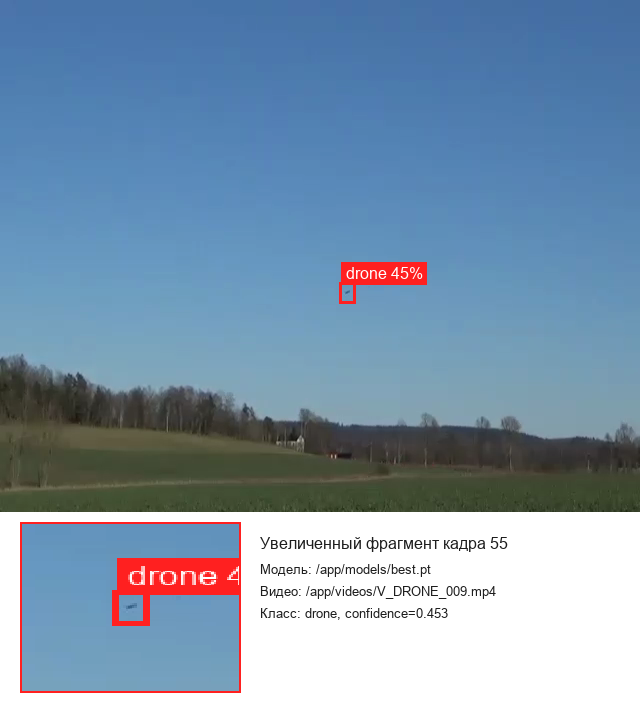
\includegraphics[width=0.92\textwidth]{../drone_demo_detection.png}
\caption{Пример детекции БПЛА на кадре 55 видео V\_DRONE\_009.mp4}
\label{fig:word_drone_demo_detection}
\end{figure}

В контрольном прогоне модель обнаружила объект класса \texttt{drone} на кадре 55 с оценкой достоверности 0.453. При работающем стеке платформа также формировала актуальные треки и события \texttt{zone\_enter}. Через API были зафиксированы треки класса \texttt{drone} с оценкой достоверности в диапазоне 0.258--0.314 и события высокого уровня важности \texttt{high}, связанные с правилом \texttt{demo-drone-zone-enter}. Это подтверждает демонстрационный путь от видеофайла и обученной модели до операторского интерфейса и журнала событий; количественные выводы по задержке и устойчивости для этого сценария требуют отдельного длительного прогона.

\begin{table}[H]
\caption{Фрагмент результатов демонстрационного прогона через API платформы}
\label{tab:drone_demo_api_results}
\begingroup
\small
\begin{tabularx}{\textwidth}{@{}>{\raggedright\arraybackslash}p{0.15\textwidth}>{\raggedright\arraybackslash}p{0.24\textwidth}>{\raggedright\arraybackslash}p{0.13\textwidth}X@{}}
\toprule
Сущность & Идентификатор & Оценка & Интерпретация \\
\midrule
Трек & \texttt{111} & 0.274 & Активный трек класса \texttt{drone}, сформированный аналитическим сервисом \\
Трек & \texttt{110} & 0.314 & Повторное обнаружение БПЛА в демонстрационном видео \\
Событие & \texttt{zone\_enter} & 0.274 & Вход БПЛА в полноэкранную демонстрационную зону контроля \\
Событие & \texttt{zone\_enter} & 0.263 & Повторная фиксация события для нового трека после дедупликации \\
\bottomrule
\end{tabularx}
\endgroup
\end{table}

Таким образом, демонстрационный контур закрывает практическую часть ВКР: обученная модель используется не изолированно, а как компонент платформы; загруженное видео применяется как воспроизводимый источник потока; результаты отображаются в интерфейсе и сохраняются в журнале событий. Это позволяет на защите показать не только качество отдельной нейросетевой модели, но и работоспособность всей платформы видеоаналитики реального времени.
